\documentclass{article}
\usepackage{amsmath}
\usepackage{graphicx}
\usepackage[utf8]{inputenc}

\title{MaS Assignment I\\
\large The Chirikov Map}
\author{Klaas Kliffen s2369494}
\date{\today}

\begin{document}

\maketitle

\section{Introduction}

The Chirikov map is defined by the set of functions:
\begin{align} 
p_{n+1} &= p_n + K \text{ sin}[2\pi x_n] / (2*\pi)\\
x_{n+1} &= x_n + p_{n+1}
\end{align}
These are taken modulo 1, to produce the following functions:
\begin{align} 
p_{n+1} &= \{p_n + K \text{ sin}[2\pi x_n] / (2*\pi)\} \text{ mod} 1\\ 
x_{n+1} &= \{x_n + p_{n+1}\} \text{ mod} 1
\end{align}

\subsection*{Initialisation}
The system is initialised by $\{x_0,p_0\} \in [0,1] \times [0,1]$

\subsection*{a) 'Orbits' in the $x$-$p$ plane for fixed $K$}
The first part of the assignment assumes a fixed value of $K = 1$ and varies the initial conditions. The aim of this part will be to distinguish between different kind of 'orbits'.

\subsection*{b) Behaviour for different values of $K$}
The second part will use the orbits from the first part and will use a varying value for $K$.
The aim of this part will be to explore the changing orbits for an increasing value of $K$


\section{Methods}
This section globally describes the adapted functions used in this assignment.

\subsection*{a) 'Orbits' in the $x$-$p$ plane for fixed $K$}
To generate the values describing the orbit, the logstep function is expanded to now accept 2 values and calculates the results from the equations 3 and 4.
This function can be used to explore the different kind of orbits given the initial values.

To plot multiple orbits for a given $K$, the logstep is called multiple times, each with different pseudo-random initial values. The calculated values are then stored in two arrays to be plotted.

\subsection*{b) Behaviour for different values of $K$}
The channelmovie is function is adapted to 'step' over $K$ instead of $r$ and to call the function to plot the orbits, rather then the channelplot.

\section{Results}

\subsection*{a: 'Orbits' in the $x$-$p$ plane for fixed $K$}

\subsection*{Points}
\begin{figure}[h!]
\centering
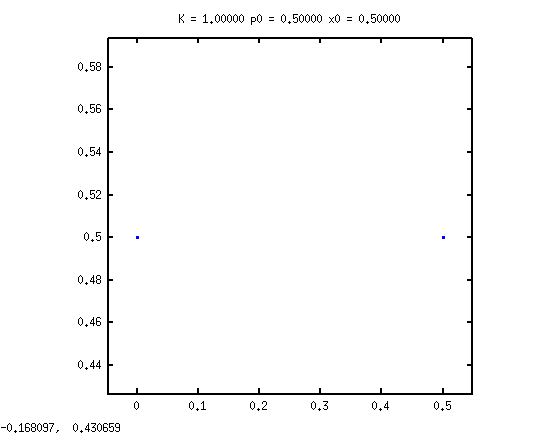
\includegraphics[width=\textwidth]{pointorbit.png}
\caption{Orbit plot of two points}
\label{pointorbit}
\end{figure}
\begin{figure}[h!]
\centering
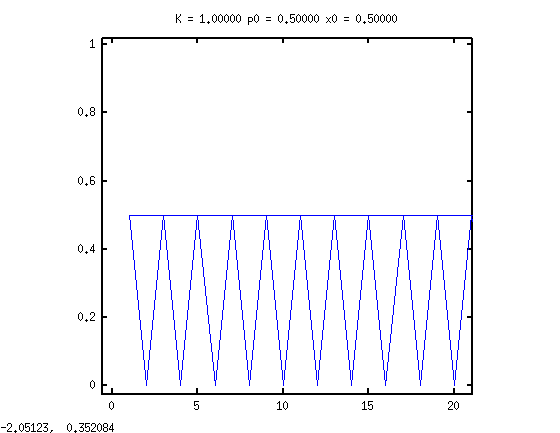
\includegraphics[width=\textwidth]{pointsvalues.png}
\caption{The values for $p$ and $x$ in the first steps }
\label{pointval}
\end{figure}

\subsection*{Curves}
\begin{figure}[h!]
\centering
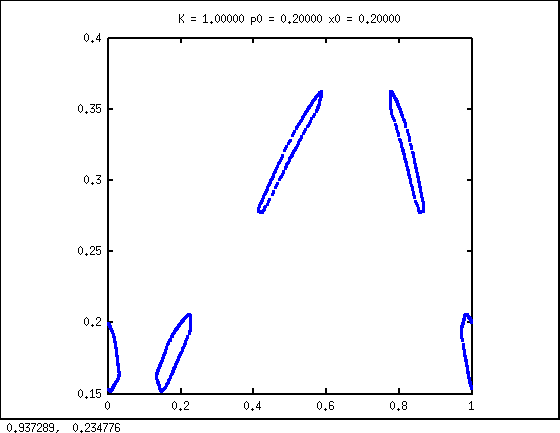
\includegraphics[width=\textwidth]{curvesorbit.png}
\caption{Orbit plot of four curves}
\label{curveorbit}
\end{figure}
\begin{figure}[h!]
\centering
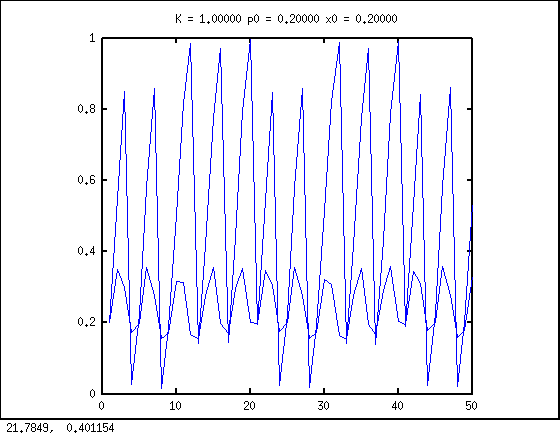
\includegraphics[width=\textwidth]{curvesvalues.png}
\caption{The values for $p$ and $x$ in the first steps }
\label{curveval}
\end{figure}

\subsection*{Areas}

\begin{figure}[h!]
\centering
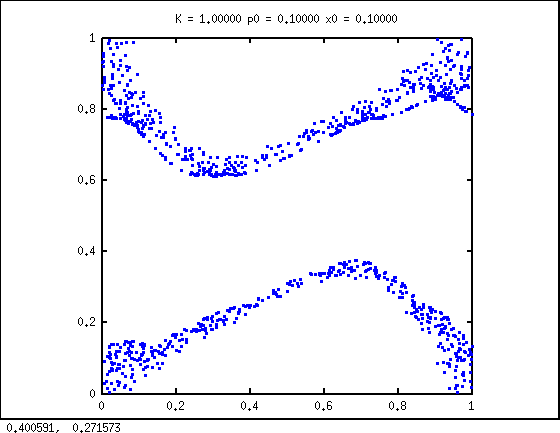
\includegraphics[width=\textwidth]{areaorbit.png}
\caption{Orbit plot of two areas}
\label{areaorbit}
\end{figure}
\begin{figure}[h!]
\centering
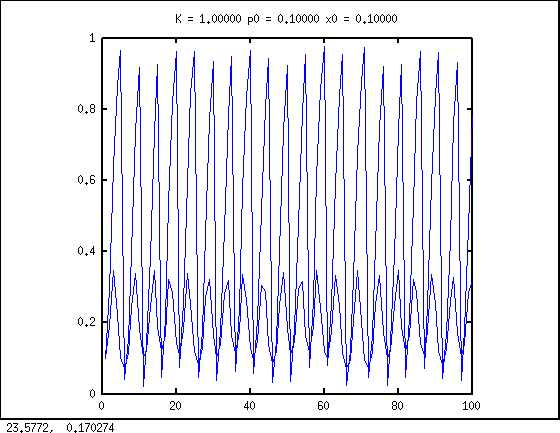
\includegraphics[width=\textwidth]{areavalues.png}
\caption{The values for $p$ and $x$ in the first steps }
\label{areaval}
\end{figure}

\subsection*{b: Behaviour for different values of $K$}

\subsubsection*{Increasing value of $K$}
Period Doubling found: curve orbits breaking into smaller curve orbits

\subsubsection*{KAM}
See reference \cite{kval} 0.971635

\begin{figure}[h!]
\centering
\begin{minipage}{0.5\textwidth}
\centering
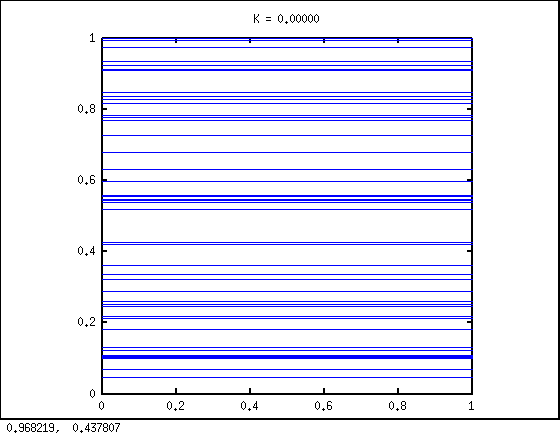
\includegraphics[width=\textwidth]{k0.png}
\caption{Orbits for $K = 0$}
\end{minipage}\hfill
\begin{minipage}{0.5\textwidth}
\centering
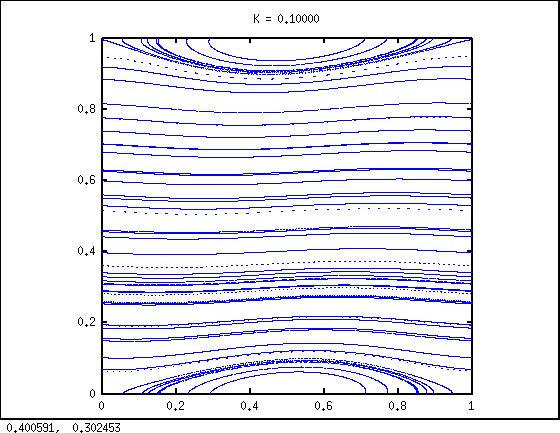
\includegraphics[width=\textwidth]{k01.png}
\caption{Orbits for $K = 0.1$}
\end{minipage}
\end{figure}

\begin{figure}[h!]
\centering
\begin{minipage}{0.5\textwidth}
\centering
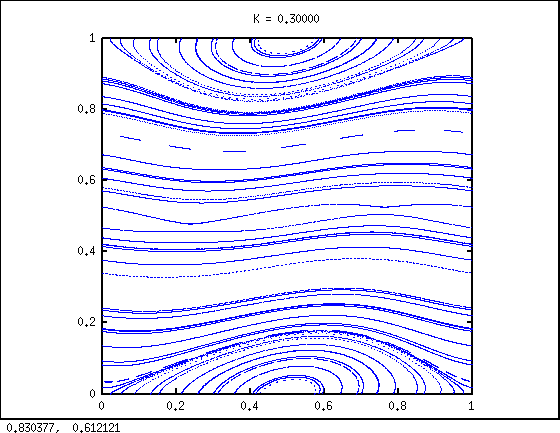
\includegraphics[width=\textwidth]{k03.png}
\caption{Orbits for $K = 0.3$}
\end{minipage}\hfill
\begin{minipage}{0.5\textwidth}
\centering
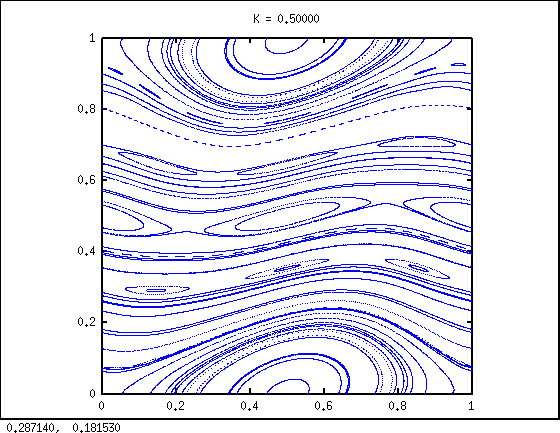
\includegraphics[width=\textwidth]{k05.png}
\caption{Orbits for $K = 0.5$}
\end{minipage}
\end{figure}

\begin{figure}[h!]
\centering
\begin{minipage}{0.5\textwidth}
\centering
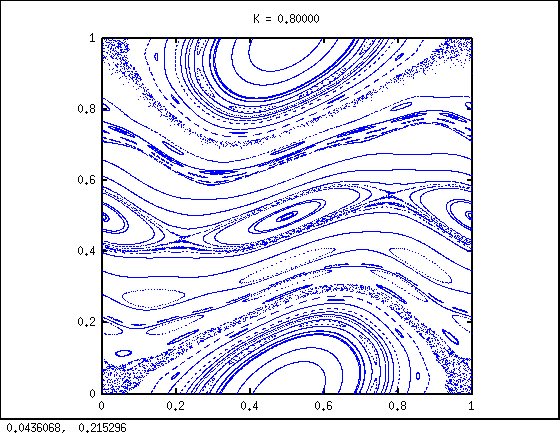
\includegraphics[width=\textwidth]{k08.png}
\caption{Orbits for $K = 0.8$}
\end{minipage}\hfill
\begin{minipage}{0.5\textwidth}
\centering
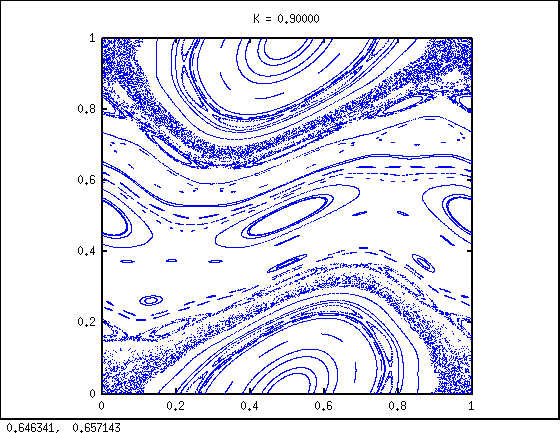
\includegraphics[width=\textwidth]{k09.png}
\caption{Orbits for $K = 0.9$}
\end{minipage}
\end{figure}

\begin{figure}[h!]
\centering
\begin{minipage}{0.5\textwidth}
\centering
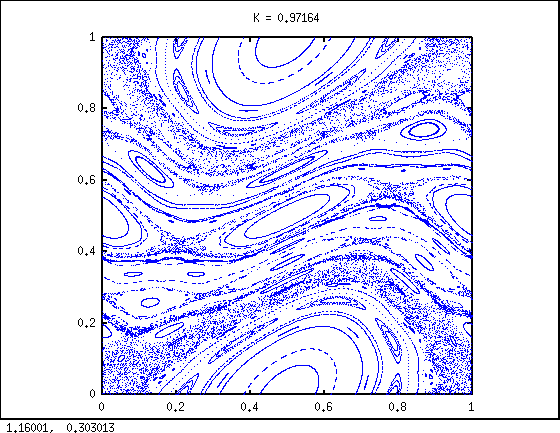
\includegraphics[width=\textwidth]{kc.png}
\caption{Orbits for $K_c = 0.97164$}
\end{minipage}\hfill
\begin{minipage}{0.5\textwidth}
\centering
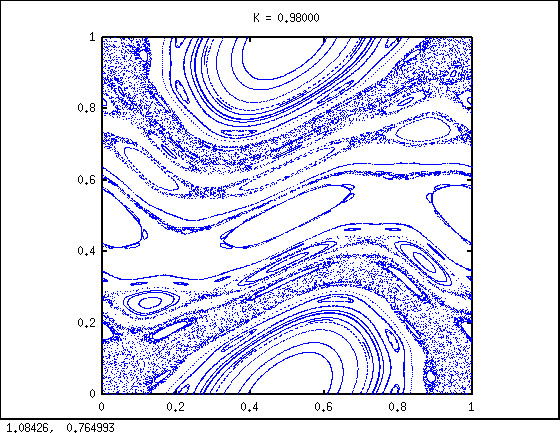
\includegraphics[width=\textwidth]{k098.png}
\caption{Orbits for $K = 0.98$}
\end{minipage}
\end{figure}

\begin{figure}[h!]
\centering
\begin{minipage}{0.5\textwidth}
\centering
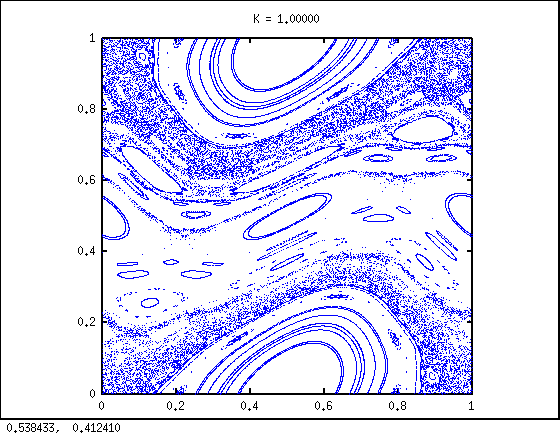
\includegraphics[width=\textwidth]{koneorbits.png}
\caption{Orbits for $K = 1.0$}
\end{minipage}\hfill
\begin{minipage}{0.5\textwidth}
\centering
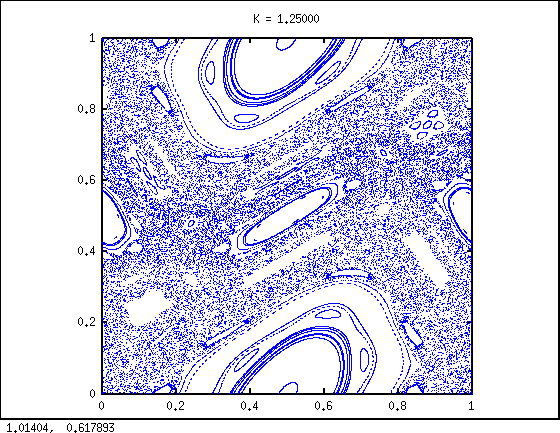
\includegraphics[width=\textwidth]{k125.png}
\caption{Orbits for $K = 1.25$}
\end{minipage}
\end{figure}

\begin{figure}[h!]
\centering
\begin{minipage}{0.5\textwidth}
\centering
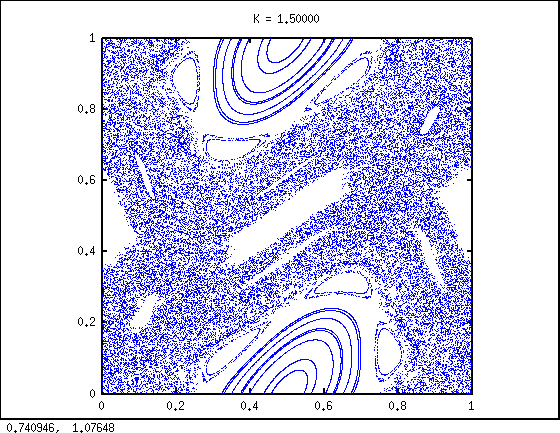
\includegraphics[width=\textwidth]{k15.png}
\caption{Orbits for $K = 1.5$}
\end{minipage}\hfill
\begin{minipage}{0.5\textwidth}
\centering
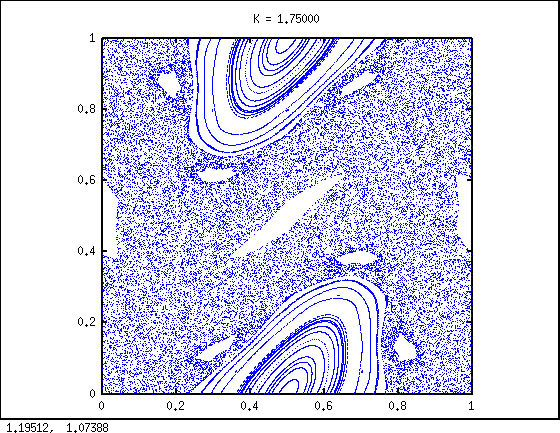
\includegraphics[width=\textwidth]{k175.png}
\caption{Orbits for $K = 1.75$}
\end{minipage}
\end{figure}

\begin{figure}[h!]
\centering
\begin{minipage}{0.5\textwidth}
\centering
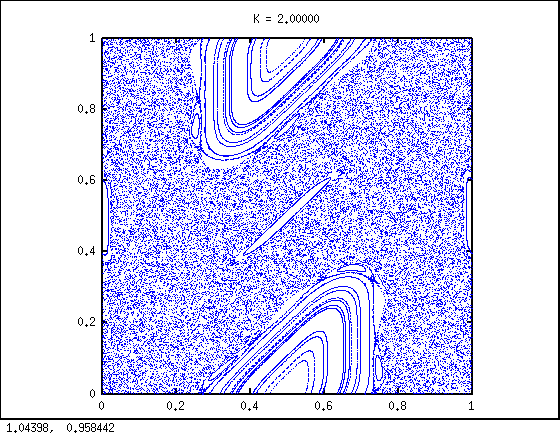
\includegraphics[width=\textwidth]{k20.png}
\caption{Orbits for $K = 2.0$}
\end{minipage}\hfill
\begin{minipage}{0.5\textwidth}
\centering
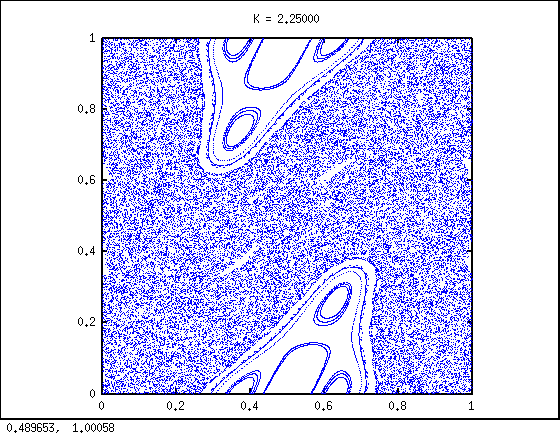
\includegraphics[width=\textwidth]{k225.png}
\caption{Orbits for $K = 2.25$}
\end{minipage}
\end{figure}

\begin{figure}[h!]
\centering
\begin{minipage}{0.5\textwidth}
\centering
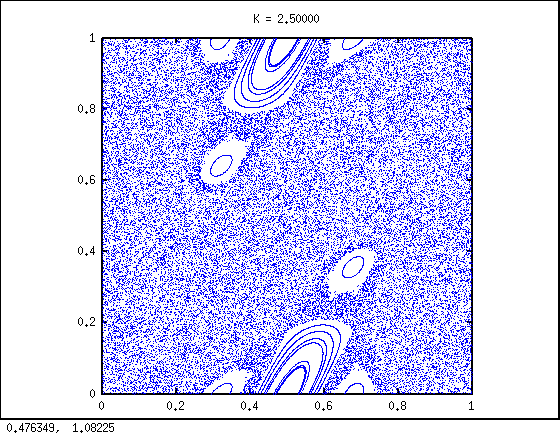
\includegraphics[width=\textwidth]{k25.png}
\caption{Orbits for $K = 2.5$}
\end{minipage}\hfill
\begin{minipage}{0.5\textwidth}
\centering
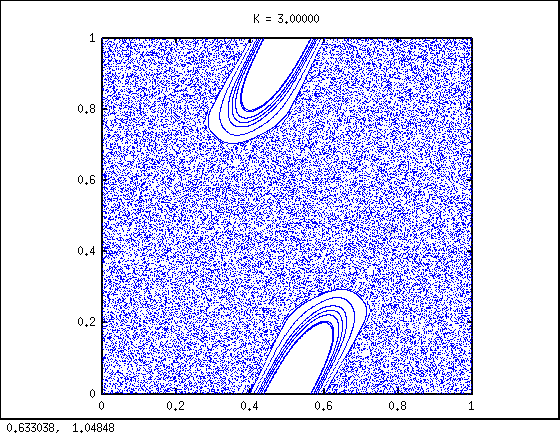
\includegraphics[width=\textwidth]{k30.png}
\caption{Orbits for $K = 3.0$}
\end{minipage}
\end{figure}


\section{Conclusion and discussion}

\subsection{a: 'Orbits' in the $x$-$p$ plane for fixed $K$}

\subsection{b: Behaviour for different values of $K$}

\subsection{Discussion}


\begin{thebibliography}{1337}
\bibitem{kval}
Greene, John M.\\
\emph{A method for determining a stochastic transition}\\
Journal of Mathematical Physics, 20, 1183-1201 (1979)\\ DOI:http://dx.doi.org/10.1063/1.524170

\end{thebibliography}
\end{document}
